\section{Computation of the SSM coefficients}\label{app:coeffs}

This appendix gives the exact recursion that produces every coefficient
$\bm w_{\bm m}$ (the geometry) and $\gamma_{2k+1}$ (the reduced dynamics) used in
the paper, matching the implementation line for line.

\subsection{Master spectral data}
Cast~\eqref{eq:eom} in first order, $\bm{\mathcal B}\dot{\bm z}=\bm{\mathcal A}\bm z
+\bm F(\bm z)$, with $\bm{\mathcal A},\bm{\mathcal B}$ as in~Sec.~\ref{sec:ssm}.
Solve the linear generalized eigenproblem $\bm K\bm\varphi=\omega_0^2\bm M\bm\varphi$,
mass-normalize $\bm\varphi^{\!\top}\bm M\bm\varphi=1$, and set
$\zeta_0=\bm\varphi^{\!\top}\bm C\bm\varphi/(2\omega_0)$. The master pencil eigenpair
solves $\bm{\mathcal A}\bm v_1=\lambda_1\bm{\mathcal B}\bm v_1$ with
$\lambda_1=-\zeta_0\omega_0+i\omega_0\sqrt{1-\zeta_0^2}$; scale $\bm v_1$ so its
displacement block is $\bm\varphi$. For symmetric $\bm M,\bm C,\bm K$ the pencil is complex-symmetric, so the left
eigenvector is $\bm u_1=\bar{\bm v}_1$ (normalized $\bm u_1^{*}\bm{\mathcal B}\bm v_1=1$);
$(\lambda_1,\bm v_1)$ is refined from the seed $([\bm\varphi;\lambda_1\bm\varphi],\lambda_1)$
by Rayleigh-quotient inverse iteration, $\bm y=(\bm{\mathcal A}-\lambda_1\bm{\mathcal B})^{-1}
\bm{\mathcal B}\bm v_1$, $\lambda_1\leftarrow\bm v_1^{\!\top}\bm{\mathcal A}\bm v_1/
\bm v_1^{\!\top}\bm{\mathcal B}\bm v_1$, which converges cubically. (A dense QZ
factorization of the first-order pencil is used only for non-symmetric systems; for the
laminated beam its master eigenvector lost up to ten digits at some ply angles.)
Set $\bm v_2=\bar{\bm v}_1$, $\lambda_2=\bar\lambda_1$. Seed the coefficient tables at first order:
$\bm w_{(1,0)}=\bm v_1$, $\bm w_{(0,1)}=\bm v_2$, $R^1_{(1,0)}=\lambda_1$,
$R^2_{(0,1)}=\lambda_2$.

\subsection{Right-hand side at each order}
For a multi-index $\bm m=(m_1,m_2)$, $|\bm m|\ge2$, the homological
equation~\eqref{eq:homological} has right-hand side
$\bm G_{\bm m}=\bm G^{\mathrm{nl}}_{\bm m}-\bm G^{\mathrm{cr}}_{\bm m}$, both assembled
from \emph{lower} orders. The nonlinear part is the order-$\bm m$ term of
$-\bm F(\bm W(\bm p))$, a multi-index convolution of the displacement blocks
$\bm w^{x}$ over all non-trivial partitions,
\begin{equation}
\bm G^{\mathrm{nl}}_{\bm m}=-\!\!\!\sum_{\substack{\bm a+\bm b=\bm m\\ \bm a,\bm b\ne\bm 0}}\!\!\!
\begin{bmatrix}\bm B_2(\bm w^{x}_{\bm a},\bm w^{x}_{\bm b})\\ \bm 0\end{bmatrix}
-\!\!\!\!\sum_{\substack{\bm a+\bm b+\bm c=\bm m\\ \bm a,\bm b,\bm c\ne\bm 0}}\!\!\!\!
\begin{bmatrix}\bm T_3(\bm w^{x}_{\bm a},\bm w^{x}_{\bm b},\bm w^{x}_{\bm c})\\ \bm 0\end{bmatrix},
\label{eq:app-forcing}
\end{equation}
and the cross-term part is what $\mathrm D\bm W\,\bm R$ already contributes from known
nonlinear reduced coefficients,
$\bm G^{\mathrm{cr}}_{\bm m}=\bm{\mathcal B}\sum_{j=1,2}\sum_{\bm a+\bm e_j=\bm m,\,|\bm b|\ge2}
a_j\,\bm w_{\bm a}R^{j}_{\bm b}$, evaluated over the already-computed $\bm w,R$.

\subsection{Solving each order}
Sweep $q=2,\dots,\text{order}$, and within each $q$ the indices $\bm m=(m_1,m_2)$ with
$m_1\ge m_2$ (the conjugate partner is filled by symmetry). Put
$\Lambda_{\bm m}=m_1\lambda_1+m_2\lambda_2$. Two cases:
\begin{itemize}
\item \textbf{Near-resonant} ($m_1-m_2=1$, i.e.\ $\bm m=(k{+}1,k)$, where
$\Lambda_{\bm m}=\lambda_1$ conservatively): the operator $\Lambda_{\bm m}\bm{\mathcal B}
-\bm{\mathcal A}$ is (near-)singular along $\bm v_1$. Project onto the left eigenvector
to read the reduced coefficient, then solve the deflated system for the geometry under
the normal-form gauge $\bm u_1^{*}\bm{\mathcal B}\bm w_{\bm m}=0$:
\begin{equation}
\boxed{\;\gamma_{2k+1}=R^1_{\bm m}=\bm u_1^{*}\bm G_{\bm m}\;},\qquad
(\Lambda_{\bm m}\bm{\mathcal B}-\bm{\mathcal A})\,\bm w_{\bm m}
=\bm G_{\bm m}-\bm{\mathcal B}\bm v_1\,R^1_{\bm m},
\label{eq:app-gamma}
\end{equation}
followed by $\bm w_{\bm m}\!\leftarrow\!\bm w_{\bm m}-(\bm u_1^{*}\bm{\mathcal B}\bm w_{\bm m})\bm v_1$.
Under light damping $\Lambda_{\bm m}\ne\lambda_1$ exactly and the solve is nonsingular; at
exact resonance one uses the least-squares pseudo-inverse and the same deflation.
\item \textbf{Non-resonant}: set $R_{\bm m}=\bm 0$ and invert directly,
$\bm w_{\bm m}=(\Lambda_{\bm m}\bm{\mathcal B}-\bm{\mathcal A})^{-1}\bm G_{\bm m}$.
\end{itemize}
The reduced coefficients are $\{\gamma_{2k+1}\}=\{R^1_{(k+1,k)}\}$ ($\gamma_3$ at
$k{=}1$, $\gamma_5$ at $k{=}2$, \dots), and the backbone is~\eqref{eq:backbone}.

\subsection{Worked coefficient: the cubic term}
At order 3 the only near-resonant index is $\bm m=(2,1)$. By~\eqref{eq:app-forcing} its
forcing is the cubic force on the master eigenvectors plus the quadratic acting on the
order-2 map, $\bm G_{(2,1)}=-\big[\,3\,\bm T_3(\bm v_1,\bm v_1,\bar{\bm v}_1)
+2\bm B_2(\bm v_1,\bm w_{(1,1)})+2\bm B_2(\bar{\bm v}_1,\bm w_{(2,0)})\,\big]$ (displacement
block), and \eqref{eq:app-gamma} gives $\gamma_3=\bm u_1^{*}\bm G_{(2,1)}$. For a
single-DOF Duffing $\ddot x+\omega_0^2x+\varepsilon x^3=0$ the quadratic vanishes, the
order-2 map is zero, and $\gamma_3$ reduces to the classical
$\Om=\omega_0\big(1+\tfrac38(\varepsilon/\omega_0^2)A^2\big)$. For the von~K\'arm\'an
plate the membrane coupling $\bm B_2$ (the $u\!\leftrightarrow\!w^2$ term) is nonzero, its
order-2 slaving $\bm w_{(1,1)},\bm w_{(2,0)}$ enters through $\bm B_2$ above, and
$\Imag\gamma_3$ equals $\tfrac{3}{2\omega_1}$ times the relaxed cubic $\gamma$ of
Eq.~\eqref{eq:gamma}, the direct membrane cubic \emph{minus} the in-plane relaxation, up to
the $O(4\omega_1^2/\omega_{\mathrm{in}}^2)$ correction of Appendix~\ref{app:ssmcond}. The
reduced coefficient \eqref{eq:app-gamma}, $\gamma_{2k+1}=\bm u_1^{*}\bm G_{(k+1,k)}$, is an
adjoint projection, which is why its design sensitivity is inexpensive.


\section{The relaxed cubic is the SSM cubic (proof of Proposition~\ref{prop:ssmcond})}\label{app:ssmcond}
Take \eqref{eq:eom} undamped with $\bm B=\bm 0$ and split $\bm x=[\bm q;\bm s]$. The linear
operators are block diagonal, so the master right eigenvector is
$\bm v_1=[\bm\varphi;\bm0;\,i\omega_1\bm\varphi;\bm0]$. Normalizing
$\bm u_1^*\bm{\mathcal B}\bm v_1=1$ with $\bm u_1=\bar{\bm v}_1$ gives the scaling
$1/(2i\omega_1)$. The quadratic force has two parts. Its $\bm s$-rows are a symmetric
form in $\bm q$, written $\bm b(\bm q,\bm q)$ (the in-plane drive of the stretch). Its
$\bm q$-rows are bilinear in $(\bm q,\bm s)$. These are the two gradients of the single
term $\int\bm\varepsilon_L^{\!\top}\bm A\bm\varepsilon_{NL}$. The cubic force acts in the
$\bm q$-rows only.

\emph{Order 2.} The forcing at $\bm m\in\{(2,0),(1,1),(0,2)\}$ has only $\bm s$-rows. Their
coefficients are $1,2,1$ times $\bm b(\bm\varphi,\bm\varphi)$, from expanding
$(p_1+p_2)^2$. The displacement-level homological equations are
\begin{equation*}
(\bm K_{\mathrm{in}}+\Lambda_{\bm m}^2\bm M_{\mathrm{in}})\,\bm s_{\bm m}=-c_{\bm m}\,\bm b(\bm\varphi,\bm\varphi),\qquad
\Lambda_{(1,1)}=0,\quad \Lambda_{(2,0)}=2i\omega_1 ,
\end{equation*}
so $\bm s_{(1,1)}=-2\bm K_{\mathrm{in}}^{-1}\bm b$ is \emph{exactly} static, while
$\bm s_{(2,0)}=-(\bm K_{\mathrm{in}}-4\omega_1^2\bm M_{\mathrm{in}})^{-1}\bm b$.

\emph{Order 3.} The resonant coefficient collects the cubic term ($3\times$) and the
quadratic $\bm q$-rows acting on $\bm s_{(1,1)}$ and $\bm s_{(2,0)}$. With static
$\bm s$, the combination is exactly $3(k_{nl}-2\bm g^{\!\top}\bm K_{\mathrm{in}}^{-1}\bm g)$,
in which $\bm s_{(1,1)}$ supplies two thirds of the relaxation and $\bm s_{(2,0)}$ one
third. Projecting with $\bm u_1$ gives $\Imag\gamma_3=\tfrac{3}{2\omega_1}\gamma$.

\emph{Error.} Expanding the resolvent,
$(\bm K_{\mathrm{in}}-4\omega_1^2\bm M_{\mathrm{in}})^{-1}=\bm K_{\mathrm{in}}^{-1}
+4\omega_1^2\bm K_{\mathrm{in}}^{-1}\bm M_{\mathrm{in}}\bm K_{\mathrm{in}}^{-1}+\dots$. This
perturbs the $(2,0)$ third of the relaxation by at most the relative amount
$\rho/(1-\rho)$, with $\rho=4\omega_1^2/\omega_{\mathrm{in}}^2$. Hence
\begin{equation*}
\Imag\gamma_3=\frac{3}{2\omega_1}(\gamma+\epsilon),\qquad
|\epsilon|\le\tfrac13\,\big(2\bm g^{\!\top}\bm K_{\mathrm{in}}^{-1}\bm g\big)\,\frac{\rho}{1-\rho}.
\end{equation*}
For the plate, $\rho=\nRhoIn$, so $|\epsilon|/\gamma<0.1\%$. In-plane inertia is
negligible for the backbone. The residual differences between \eqref{eq:gamma} and the
full SSM in Sec.~\ref{sec:confirm} come from the transverse basis, not from the
condensation.

\section{Finite-element validation of the assumed-modes discretization}\label{app:fe}

\paragraph{Why this is needed.} The reductions above are verified against the analytic
Duffing backbone and against full-order EPMC and direct time integration. Those
confirmations, however, are of the \emph{same} assumed-modes system solved at higher
fidelity: they validate the SSM \emph{reduction}, not the assumed-modes
\emph{discretization}. A steered laminate is spatially heterogeneous and, off the
principal axes, develops bend--twist couplings $D_{16},D_{26}$; whether a handful of
global sine modes resolve its response is a separate question. We settle it with an
independent finite-element (FE) model and the identical backbone coefficient.

\subsection{FE model}
We take a flat, symmetric ($\bm B=\bm0$) plate on a uniform $n_x\times n_y$ rectangular
mesh, bending and membrane discretized independently (they decouple linearly for
$\bm B=\bm 0$).

\emph{Bending (Kirchhoff).} The non-conforming 12-DOF ACM rectangular element carries
nodal degrees of freedom $\bm d_e=\{w,\;w_{,y},\;-w_{,x}\}$ at the four corners. On the
element (local $s,t\in[0,1]$) the deflection is the 12-term polynomial
\begin{equation}
w(s,t)=\bm p^{\!\top}\bm a,\quad
\bm p=[1,s,t,s^2,st,t^2,s^3,s^2t,st^2,t^3,s^3t,st^3]^{\!\top};
\end{equation}
enforcing the nodal DOF gives $\bm d_e=\bm C\bm a\Rightarrow\bm a=\bm C^{-1}\bm d_e$. With
the curvature $\bm\kappa=[w_{,xx},w_{,yy},2w_{,xy}]^{\!\top}=\bm B_b\bm C^{-1}\bm d_e$
($\bm B_b$ the side-scaled second derivatives of $\bm p$), and $4\times4$ Gauss quadrature,
\begin{equation}
\bm K^b_e=\!\int_{\Omega_e}\!\bm C^{-\top}\bm B_b^{\!\top}\,\bm D(\theta_e)\,\bm B_b\bm C^{-1}\,\dd\Omega,
\quad
\bm M^b_e=\rho h\!\int_{\Omega_e}\!\bm C^{-\top}\bm p\bm p^{\!\top}\bm C^{-1}\,\dd\Omega,
\end{equation}
$\bm D(\theta_e)=\tfrac{h^3}{12}\bar{\bm Q}(\theta_e)$ evaluated per element, so
$D_{16},D_{26}$ are retained exactly.

\emph{Membrane (Q4).} The in-plane fields use the 8-DOF bilinear quadrilateral; with the
membrane strain--displacement $\bm B_m$ and $\bm A(\theta_e)=h\,\bar{\bm Q}(\theta_e)$,
$\bm K^{\mathrm{in}}_e=\int_{\Omega_e}\bm B_m^{\!\top}\bm A(\theta_e)\bm B_m\,\dd\Omega$.

\emph{Boundary conditions.} Navier simple support: $w=0$ on the boundary (bending) and
$u=v=0$ on the boundary (membrane) --- matching the sine in-plane modes, which vanish on
the edges. \emph{Self-validation:} for a specially-orthotropic UD $[0]$ plate the FE
reproduces the closed form
$\omega_{mn}=\pi^2\sqrt{[D_{11}(m/a)^4+2(D_{12}{+}2D_{66})(m/a)^2(n/b)^2+D_{22}(n/b)^4]/\rho h}$
to $f_1=\nFEselfUD$ vs.\ $\nUDf$~Hz, converging monotonically with mesh
(\texttt{examples/plate\_fe\_check.py}).

\subsection{Backbone by static condensation on the mesh}
We compute the \emph{same} backbone coefficient the plate results use ---
Eq.~\eqref{eq:gamma} --- but FE-discretized. Solve $\bm K^b\bm\varphi=\omega_1^2\bm M^b\bm\varphi$
for the fundamental mode (unit peak deflection); its von~K\'arm\'an membrane strain is
$\bm\varepsilon_{NL}=[\tfrac12 w_{,x}^2,\tfrac12 w_{,y}^2,w_{,x}w_{,y}]^{\!\top}$, with the
gradients read off the ACM element. Assembling
$\bm g=\!\int\bm B_m^{\!\top}\bm A\,\bm\varepsilon_{NL}$,
$\mathrm{knl}=2\!\int\bm\varepsilon_{NL}^{\!\top}\bm A\,\bm\varepsilon_{NL}$ and
$K_b=\bm\varphi^{\!\top}\bm K^b\bm\varphi$, static condensation of the fast in-plane fields gives
\begin{equation}
\gamma=\mathrm{knl}-2\,\bm g^{\!\top}(\bm K^{\mathrm{in}})^{-1}\bm g,
\qquad
\Om(a)/\omega_1=1+\beta\,(a/h)^2,\quad \beta=\tfrac38\,(\gamma/K_b)\,h^2 .
\end{equation}
This costs \emph{one} sparse solve --- no continuation or time integration --- because the
condensation \emph{is} the order-2 SSM slaving (App.~\ref{app:coeffs}) evaluated on the mesh.
The identical formula on the sine basis returns the assumed-modes backbone, so any difference
is purely discretization (\texttt{examples/plate\_fe\_backbone.py}).

\subsection{Results}
Table~\ref{tab:fe} compares the two discretizations for a homogeneous and a strongly steered
field ($\theta=20^\circ+45^\circ\sin\tfrac{\pi x}{a}\sin\tfrac{\pi y}{b}$, sweeping
$20^\circ$--$65^\circ$).

\begin{table}[!tbp]
\centering\footnotesize
\IfFileExists{fe_table.tex}{\begin{tabular}{llccc}
\toprule
field & model & $f_1$ [Hz] & $\gamma$ & detuning @ $a/h{=}0.4$\\
\midrule
UD $[0]$ (homogeneous) & FE ($28\times21$) & $256.0$ & $2.878\!\times\!10^{10}$ & $11.06\%$\\
 & assumed-modes & $256.3$ & $2.842\!\times\!10^{10}$ & $10.96\%$ \;($1\%$)\\
\midrule
steered (strong) & FE ($28\times21$) & $334.4$ & $2.515\!\times\!10^{10}$ & $5.73\%$\\
 & assumed, $8$ modes & $358.9$ & $2.546\!\times\!10^{10}$ & $5.30\%$ \;($7\%$)\\
 & assumed, $24$ modes & $345.7$ & $2.584\!\times\!10^{10}$ & $5.65\%$ \;($2\%$)\\
\bottomrule
\end{tabular}
}{\textit{table pending}}
\caption{Assumed-modes vs.\ FE backbone (parenthesized: detuning error vs.\ FE). ``$N$
modes'' is the number of transverse modes in total (the $N$ lowest), with $3\times3$
in-plane modes; the design evaluator uses 64 transverse ($m,n\le8$) and $6\times6$ in-plane
modes (Table~\ref{tab:conv}). This test therefore checks the transverse discretization
and the nonlinear FE model on a smooth steered field ($20^\circ$--$65^\circ$); the in-plane
resolution of the actual design is checked separately by the FE evaluation of the
optimized field (ratio $\nFEratio$, Sec.~\ref{sec:confirm}). Homogeneous:
the two agree to $\nFEtabUDagree\%$, validating the FE nonlinear model. Strong steering: the frequency is a
slowly-converging Ritz upper bound ($+\nFEtabFreqErrEight\%$ at $8$ modes, $+\nFEtabFreqErrTwentyFour\%$ at $24$), but the
\emph{normalized detuning} --- the design quantity --- matches FE to $\nFEtabDetErrEight\%$ at $8$ modes and
$\nFEtabDetErrTwentyFour\%$ at $24$.}
\label{tab:fe}
\end{table}

\begin{figure}[!tbp]
\centering
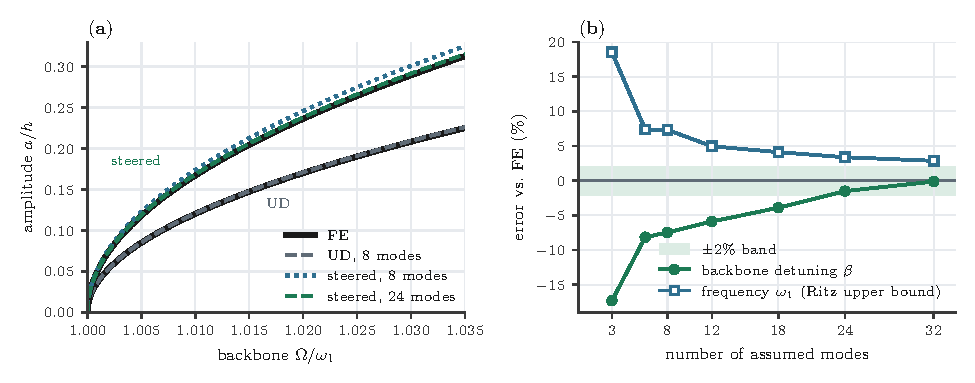
\includegraphics[width=\linewidth]{figs/plate_fe_validation.pdf}
\caption{\textbf{The assumed-modes backbone agrees with an independent finite-element model.}
\textbf{(a)}~Amplitude vs.\ backbone frequency (same orientation as
Figs.~\ref{fig:beam} and \ref{fig:confirm}); black: FE. For the homogeneous UD plate the
8-mode assumed-modes backbone (gray dashed) coincides with FE, validating the FE nonlinear
model; for the strongly steered plate the assumed-modes backbone converges to FE as modes
are added (8 modes dotted, 24 modes green dashed, overlying FE). \textbf{(b)} Ritz convergence toward FE (steered): the normalized
backbone detuning enters the $\pm2\%$ band by $\sim\!24$ modes, whereas the absolute frequency is
a slowly-converging Ritz upper bound. The design quantity (relative detuning) is the well-resolved
one.}
\label{fig:fe}
\end{figure}

Two conclusions. \emph{(i)} For a homogeneous laminate the FE and assumed-modes backbones
agree to $\nFEtabUDagree\%$, validating the FE nonlinear model (membrane, coupling, condensation).
\emph{(ii)} For strong steering the assumed-modes frequency is a Ritz upper bound that
converges slowly, but the \emph{normalized backbone detuning} $\beta\propto\gamma/K_b$
is far more robust --- a ratio of two integrals of the \emph{same} slightly-inaccurate mode, so
the mode-shape error largely cancels, leaving a $\nFEtabDetErrTwentyFour\%$ discrepancy at $24$ modes. The relative
detuning results the designs are built on are therefore FE-accurate to a few percent; absolute
frequencies of strongly steered designs should be read from FE or an enriched
($\gtrsim24$-mode) expansion. The paper's design evaluator uses 64 transverse modes, and the
optimized design itself is evaluated on this FE model in Sec.~\ref{sec:confirm} (detuning
ratio $\nFEratio$ vs.\ $\nCratioSSM$ from the full SSM). A displacement-based von~K\'arm\'an FE would replace the assumed
modes throughout at higher cost, reduced by the same SSM.


\section{Calibration against prior work, and SSM- vs EPMC-driven optimization}\label{app:calib}
We reproduce two published results of \cite{pozzi2025} as a check of the reduction and
its sensitivities, and compare SSM- and EPMC-driven optimization on one benchmark.
\emph{(i)} The backbone sensitivity of two coupled oscillators predicts the perturbed
backbone to within about $3\times10^{-5}$ in $\Om$ over its soften-then-harden shape (the
frequency first falls, then turns back up near an RMS amplitude of 1). Capturing the
turn-back needs a high-order SSM; we use order seven, where \cite{pozzi2025} use order
five with an analytic adjoint (Fig.~\ref{fig:fig2}). The damped eigenvalue
$\lambda=-0.0191\pm0.6177i$ matches exactly. \emph{(ii)} A clamped von K\'arm\'an beam
is shaped by an initial curvature to a prescribed softening backbone, and full-order
EPMC confirms the optimized SSM backbone to $<0.1\%$ (Fig.~\ref{fig:fig3}). Two
departures are noted. First, we use the axially condensed shallow-arch model rather
than a three-DOF-per-node element. Second, we place the target amplitudes inside the
cubic SSM's verified window. Eq.~(33) of \cite{pozzi2025}, taken literally, places a
same-sign quadratic coupling on both masses, which is not energy-consistent; the
potential-derived spring we use leaves the reported eigenvalue unchanged.

\paragraph{Validity window of the cubic SSM.} Over the amplitudes reached by the
full-order EPMC continuation ($a/h\le\nEPMCmaxUD$ for UD, $\le\nEPMCmaxOpt$ for the steered design;
Fig.~\ref{fig:confirm}a), the cubic SSM backbone reproduces the EPMC detuning
$\Om/\omega_1-1$ to within $\nEPMCAgree\%$. The jump thresholds compared in
Sec.~\ref{sec:jumpres} ($a_c/h=\nCUDac$ and $\nCOptac$) lie inside these ranges; we make no
claim beyond them, where higher-order terms bend the true backbone.

\begin{figure}[!tbp]
\centering
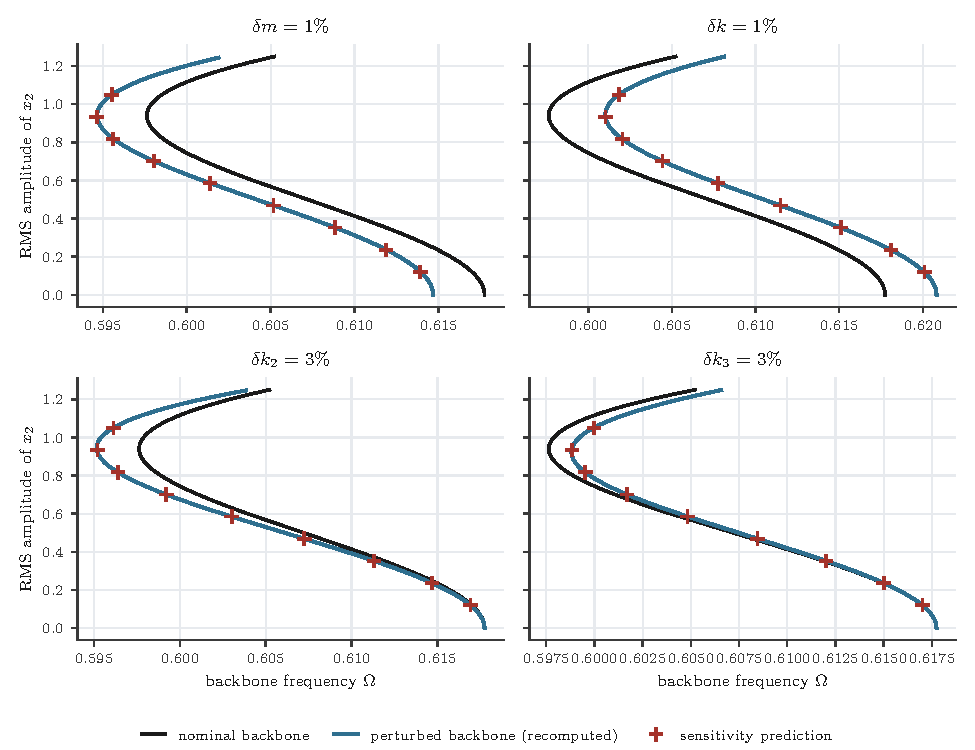
\includegraphics[width=\linewidth]{figs/coupled_osc_sensitivity.pdf}
\caption{\textbf{The backbone sensitivities reproduce a published benchmark.} Calibration against
\cite{pozzi2025}, Fig.~2: backbone-sensitivity
validation of two coupled oscillators. Each panel perturbs one parameter
($m$, $k$: $1\%$; $k_2$, $k_3$: $3\%$). Black: nominal backbone; blue: perturbed backbone,
recomputed; red crosses: first-order sensitivity prediction from the nominal backbone. The
predictions land on the recomputed backbones through the soften-then-harden turn-back,
which the seventh-order SSM captures.}
\label{fig:fig2}
\end{figure}

\begin{figure}[!tbp]
\centering
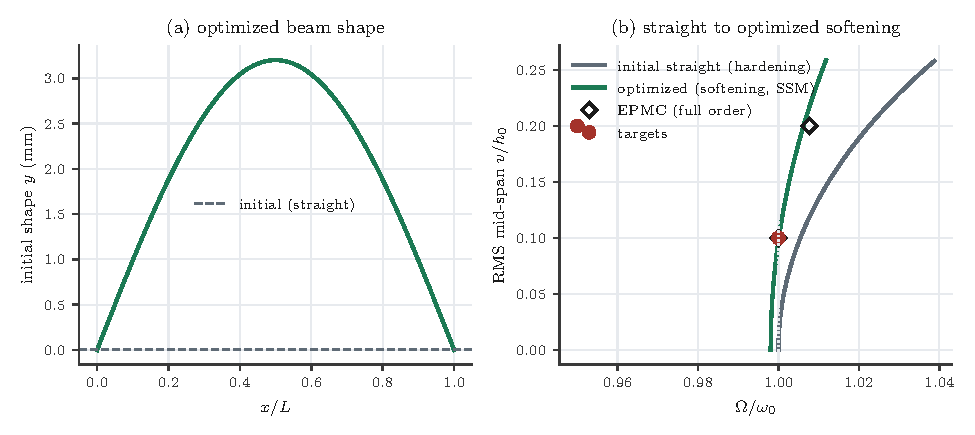
\includegraphics[width=\linewidth]{figs/beam_backbone_opt.pdf}
\caption{\textbf{The SSM design loop reproduces a published backbone-shaping result.} Calibration
against \cite{pozzi2025}, Fig.~3: a von~K\'arm\'an beam
shaped to a prescribed softening backbone. This problem shapes the beam with up to two harmonics (the optimum uses only the first)
to pass through two prescribed backbone points; it is a different problem from that of
Fig.~\ref{fig:svse}, which tunes one amplitude to one target. \textbf{(a)}~Optimized
initial shape $y(x)$ and the straight starting design.
\textbf{(b)}~Backbones, normalized by the first frequency $\omega_{1,0}$ of the initial
straight beam: the straight (hardening) beam becomes a curved (softening) one threading
both target points; full-order EPMC (diamonds) confirms the optimized SSM backbone to
$<0.1\%$.}
\label{fig:fig3}
\end{figure}

\paragraph{EPMC as a design engine.} The extended periodic motion concept
\cite{krack2015} augments the equation of motion with a self-excitation that offsets
damping, $\bm M\ddot{\bm q}+(\bm C-2\delta\Om\bm M)\dot{\bm q}+\bm K\bm q+\bm f_{nl}=\bm0$,
and continues the harmonic-balance residual $\bm R(\bm z;a,\theta)=\bm0$ in amplitude.
Its design sensitivity at a converged point follows from the implicit-function theorem
with the Newton Jacobian already assembled, through one adjoint solve per amplitude,
$\dd\Om/\dd\theta=-\bm w^{\!\top}\partial_\theta\bm R$ with $\bm J_z^{\!\top}\bm w=\bm e_\Om$.
$\partial_\theta\bm R$ reuses the same $\partial\bar{\bm Q}/\partial\theta$ as the SSM
gradient. The two engines are complementary. The SSM gives a smooth, analytic objective
at a cost independent of amplitude and harmonic count, and is the search engine here.
EPMC is exact at any amplitude it reaches, captures folds and internal resonances, and
serves as the validation of record. On the benchmark below, both find nearly the same
optimum, and the SSM backbone is about two orders of magnitude cheaper per evaluation.

\subsection{SSM- and EPMC-driven optimization on the same benchmark}
To compare the two engines as \emph{optimizers}, we solve the same design problem
with each on the published von~K\'arm\'an-beam backbone-shaping benchmark of
\cite{pozzi2025} (their Sec.~5.2 / Fig.~3): a clamped--clamped beam whose backbone
is shaped from hardening to a prescribed \emph{softening} by an initial curvature
$y=A_1\sin(\pi x/L)$. The straight beam hardens ($+2.2\%$ relative detuning at
$\mathrm{RMS}=0.2h_0$); the curvature injects a quadratic nonlinearity whose slaved
response drives the SSM cubic coefficient negative, softening the backbone (it also
stiffens the beam linearly, so the curvature-invariant measure is the detuning
relative to each design's \emph{own} $\omega_1$). We design $A_1$ to hit a $-1.5\%$
softening target, driving the optimizer once with the SSM backbone and once with the
full-order EPMC backbone. Both reach the target exactly. The optima are $A_1=8.03$\,mm
(SSM) and $8.26$\,mm (EPMC), a $2.8\%$ difference that is the cubic SSM's truncation
error at $\mathrm{RMS}=0.2h_0$. The SSM backbone costs about two orders of magnitude less per
evaluation (Fig.~\ref{fig:svse}). This is the intended division of labor: the SSM adjoint does
the search cheaply, and full-order EPMC confirms the optimum.

\begin{figure}[!tbp]
\centering
\begin{minipage}[c]{0.54\linewidth}\centering
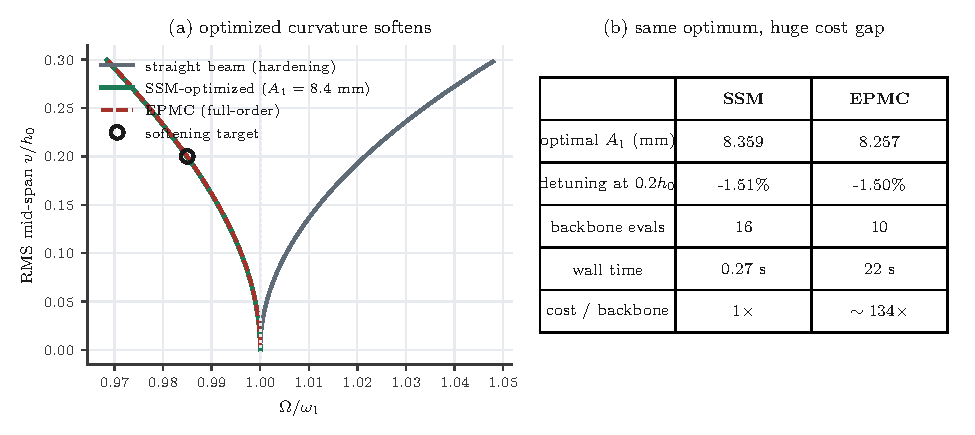
\includegraphics{figs/ssm_vs_epmc_opt.pdf}
\end{minipage}\hfill
\begin{minipage}[c]{0.43\linewidth}\centering\footnotesize
(\textbf{b})\\[4pt]
\IfFileExists{svse_table.tex}{\begin{tabular}{@{}lrr@{}}
\toprule
 & SSM & EPMC\\ \midrule
optimal $A_1$ (mm) & 8.03 & 8.26\\
detuning at $0.2h_0$ & $-1.50\%$ & $-1.50\%$\\
backbone evaluations & 12 & 10\\
wall time (s) & 0.059 & 11.2\\
cost per backbone & $1\times$ & $\approx230\times$\\
\bottomrule
\end{tabular}
}{\textit{table pending}}
\end{minipage}
\caption{\textbf{SSM- and EPMC-driven optimization reach nearly the same optimum, at very different
cost.} Optimizing the same design with both frameworks (benchmark of
\cite{pozzi2025}). Here one curvature amplitude $A_1$ is tuned to one softening
target (a different problem from Fig.~\ref{fig:fig3}). \textbf{(a)}~The straight beam's
backbone hardens (leans right); the
optimized initial curvature softens it (leans left) through the softening target; the
SSM- and EPMC-optimized backbones nearly coincide. \textbf{(b)}~The two optima and
their cost; the SSM optimum differs from the full-order one by the cubic SSM's
truncation error at $\mathrm{RMS}=0.2h_0$, at about two orders of magnitude lower cost
per backbone evaluation (wall times are indicative only).}
\label{fig:svse}
\end{figure}




\section{Verification and reproducibility}\label{app:repro}
Every computed result quoted in the main text and in Appendices A--C is a macro generated
from the result files by \texttt{examples/paper\_numbers.py} (\texttt{docs/paper/numbers.tex}),
or a table written by a listed script; the few rounded bounds and estimates stated in words
(e.g.\ ``less than $0.02$'', the bang-bang estimate $0.4$--$0.5$) follow from those values. The calibration values of Appendix~\ref{app:calib} (the replicated
benchmarks of \cite{pozzi2025}) are printed by the scripts listed for them below. Table~\ref{tab:repro}
maps each result to the script that produces it. Unit tests are in \texttt{tests/}
(\texttt{pytest}).

\begin{table}[!tbp]
\centering\footnotesize
\caption{Result $\to$ script map.}\label{tab:repro}
\begin{tabular}{@{}>{\raggedright\arraybackslash}p{0.42\linewidth}>{\raggedright\arraybackslash}p{0.54\linewidth}@{}}
\toprule
result & script (in \texttt{examples/} unless a path is given)\\ \midrule
relaxed evaluator, gradient, tests & \texttt{nltopt/relaxed\_plate.py}, \texttt{tests/test\_relaxed\_plate.py}\\
beam test (Sec.~\ref{sec:beamres}, Fig.~\ref{fig:beam}) & \texttt{beam\_symmetric\_steering.py}, \texttt{fig\_beam.py}\\
$B$-coupled beam (comparison) & \texttt{steered\_beam\_amplitude\_robust.py}\\
achievable sets (Sec.~\ref{sec:levers}, Fig.~\ref{fig:levers}) & \texttt{levers\_study.py}, \texttt{fig\_levers.py}\\
mechanism, front, dose (Figs.~\ref{fig:mechanism}, \ref{fig:limits}) & \texttt{mechanism\_study.py}, \texttt{fig\_mechanism.py}, \texttt{fig\_limits.py}\\
resolution and pointwise ceiling & \texttt{ceiling\_study.py}\\
full-order confirmation (Sec.~\ref{sec:confirm}), jump (Sec.~\ref{sec:jumpres}) & \texttt{confirm\_heldfreq.py} (SSM, thresholds, sweeps), then \texttt{epmc\_check.py} (merges the EPMC backbones into the same file), \texttt{confirm\_fine\_sweep.py}, \texttt{fig\_confirm.py}\\
independent FE check of the design (Table~\ref{tab:confirm}) & \texttt{fe\_check\_design.py}\\
basis convergence (Table~\ref{tab:conv}) & \texttt{conv\_table.py}\\
continuous-stack competitor (Sec.~\ref{sec:levers}) & \texttt{stack\_continuous.py}\\
frequency multiplier, linear spectra (Secs.~\ref{sec:mechanism}, \ref{sec:discussion}) & \texttt{mechanism\_lambda.py}, \texttt{mode\_ratios.py}\\
all quoted numbers and generated tables & \texttt{paper\_numbers.py}\\
FE validation (App.~\ref{app:fe}) & \texttt{plate\_fe\_backbone.py}, \texttt{plate\_fe\_fig.py}\\
calibration (App.~\ref{app:calib}) & \texttt{coupled\_osc\_sensitivity.py}, \texttt{beam\_backbone\_opt.py}, \texttt{ssm\_vs\_epmc\_opt.py}\\
matched-frequency comparison (Sec.~\ref{sec:confirm}, Fig.~\ref{fig:levers}b) & \texttt{r1\_matched\_frequency.py}\\
other plates, conflict (Sec.~\ref{sec:robust}, Fig.~\ref{fig:robust}a,b) & \texttt{r1\_generality.py}, \texttt{r1\_conflict.py}\\
damping level and law (Fig.~\ref{fig:robust}c) & \texttt{r1\_damping.py}\\
as-built tow defects (Sec.~\ref{sec:asbuilt}, Fig.~\ref{fig:robust}d,e) & \texttt{r1\_asbuilt.py}, \texttt{fig\_robust.py}\\
gradient, independent-grid and multi-start checks (Table~\ref{tab:ms}) & \texttt{r1\_verification.py}\\
\bottomrule
\end{tabular}
\end{table}
